\section{Quicksort}
Es wird oft gewünscht, dass Daten sortiert vorliegen. Dabei ist es in der Regel gleichwertig, ob sie aufsteigend alphabetisch, absteigend oder nach anderen Kriterien sortiert werden.

Sortieralgorithmen sind daher ein häufiges Thema in der Informatik. Bubblesort ist einfach zu erlernen, aber relativ langsam. Bei großen Datenmengen wird Bubblesort eher nicht verwendet.

Quicksort wird häufiger verwendet. Der Algorithmus ist relativ schnell in der Ausfüh\-rung. Quicksort kann in verschiedenen Varianten implementiert werden. Ich verwende die sogenannte in-Place-Variante, bei der zwei Zeiger die Elemente absuchen und direkt vertauschen, falls nötig.

Im Beispiel möchte ich das folgende Array mit Zahlen sortieren lassen.
\begin{figure}
  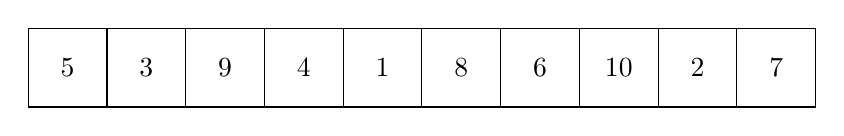
\begin{tikzpicture}
    \foreach \x in {1,...,10}
      \draw (\x,0) +(-.5,-.5) rectangle ++(.5,.5);
      \draw (1,0) node{5};
      \draw (2,0) node{3};
      \draw (3,0) node{9};
      \draw (4,0) node{4};
      \draw (5,0) node{1};
      \draw (6,0) node{8};
      \draw (7,0) node{6};
      \draw (8,0) node{10};
      \draw (9,0) node{2};
      \draw (10,0) node{7};
  \end{tikzpicture}
  \caption{Array, Ausgangssituation}
  \label{quicksortArrayAusgang}
\end{figure}

\subsection{Quicksort, Version in-place}
Im ersten Schritt wird ein Pivotelement festgelegt. Das Element wird später benötigt, um andere Einträge mit dem Pivotelement zu vergleichen. Im ersten Schritt ist es gleichgültig, ob ich das erste oder letzte Element wähle. Ich wähle das letzte Element des Arrays (siehe Bild \ref{quicksortArrayPivot_1}).

\begin{figure}
  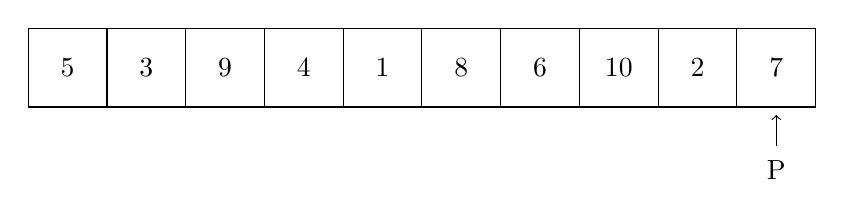
\begin{tikzpicture}
    \foreach \x in {1,...,10}
      \draw (\x,0) +(-.5,-.5) rectangle ++(.5,.5);
      \draw (1,0) node{5};
      \draw (2,0) node{3};
      \draw (3,0) node{9};
      \draw (4,0) node{4};
      \draw (5,0) node{1};
      \draw (6,0) node{8};
      \draw (7,0) node{6};
      \draw (8,0) node{10};
      \draw (9,0) node{2};
      \draw (10,0) node{7};
      \draw [->](10,-1) -- (10,-0.6);
      \draw (10,-1.3) node{P};
  \end{tikzpicture}
  \caption{Array, Ausgangssituation}
  \label{quicksortArrayPivot_1}
\end{figure}

Jetzt werden zwei Hilfszeiger benötigt (klein und gross). Gross (g) beginnt am linken Ende des Arrays, klein (k) am rechten neben dem Pivotelement (siehe Bild \ref{quicksortArrayP_k_g_11}). In jedem Arbeitsschritt prüfe ich, ob die Stelle bei klein kleiner ist als das Pivotelement und gross größer oder gleich groß gegenüber dem Pivotelement ist. Falls klein kleiner oder gleich ist im Vergleich zum Pivotelement lasse ich es an der Position stehen und setze den Suchzeiger (k) um eine Position weiter nach rechts. Falls ich ein Element finde, das größer als der Pivotelement ist, lasse ich den Suchzeiger k dort stehen und suche mit gross (g) nach einem Element, das kleiner oder gleich gegenüber dem Pivotelement ist.

\begin{figure}
  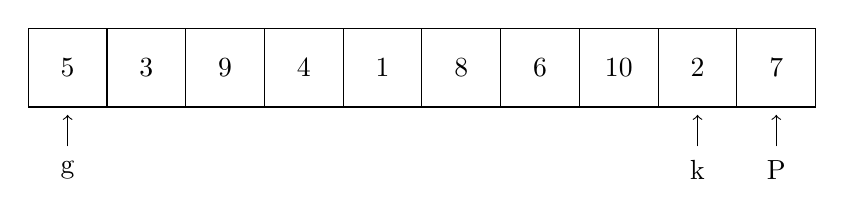
\begin{tikzpicture}
    \foreach \x in {1,...,10}
      \draw (\x,0) +(-.5,-.5) rectangle ++(.5,.5);
      \draw (1,0) node{5};
      \draw (2,0) node{3};
      \draw (3,0) node{9};
      \draw (4,0) node{4};
      \draw (5,0) node{1};
      \draw (6,0) node{8};
      \draw (7,0) node{6};
      \draw (8,0) node{10};
      \draw (9,0) node{2};
      \draw (10,0) node{7};
      \draw [->](10,-1) -- (10,-0.6);
      \draw (10,-1.3) node{P};
      \draw [->](1,-1) -- (1,-0.6);
      \draw (1,-1.3) node{g};
      \draw [->](9,-1) -- (9,-0.6);
      \draw (9,-1.3) node{k};
 \end{tikzpicture}
  \caption{Array, Zeiger auf kleineres und größeres Element (relativ zu Pivotelement)}
  \label{quicksortArrayP_k_g_11}
\end{figure}

Im Beispiel sucht der Zeiger \glq g\grq \ zuerst von links kommend das erste Element, das größer als 7 ist. Anschließend sucht k das nächste Element, das kleiner oder gleich 7 ist (Bild \ref{quicksortArrayP_k_g_12}). Hier entsprechen die Werte 5 und 2 an den ersten Positionen von g und k den Kriterien der Suche.

\begin{figure}
  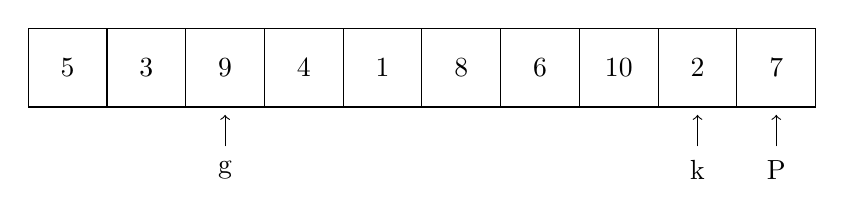
\begin{tikzpicture}
    \foreach \x in {1,...,10}
      \draw (\x,0) +(-.5,-.5) rectangle ++(.5,.5);
      \draw (1,0) node{5};
      \draw (2,0) node{3};
      \draw (3,0) node{9};
      \draw (4,0) node{4};
      \draw (5,0) node{1};
      \draw (6,0) node{8};
      \draw (7,0) node{6};
      \draw (8,0) node{10};
      \draw (9,0) node{2};
      \draw (10,0) node{7};
      \draw [->](10,-1) -- (10,-0.6);
      \draw (10,-1.3) node{P};
      \draw [->](3,-1) -- (3,-0.6);
      \draw (3,-1.3) node{g};
      \draw [->](9,-1) -- (9,-0.6);
      \draw (9,-1.3) node{k};
 \end{tikzpicture}
  \caption{Array, Zeiger auf Elemente zum Tausch}
  \label{quicksortArrayP_k_g_12}
\end{figure}

Im folgenden Schritt werden die Einträge, auf die g und k zeigen, vertauscht. Anschließend sucht der Algorithmus wieder, solange, bis die Hilfszeiger wieder passende Elemente gefunden haben. Falls g und k bei der Suche aneinander vorbeilaufen, bricht der Such- und Vertauschungs-Algorithmus ab. In Bild \ref{quicksortArrayP_k_g_13} stehen 8 und 6 zum Tauscht an. %Anschließend tauschen die Hilfszeiger die Positionen.

\begin{figure}
  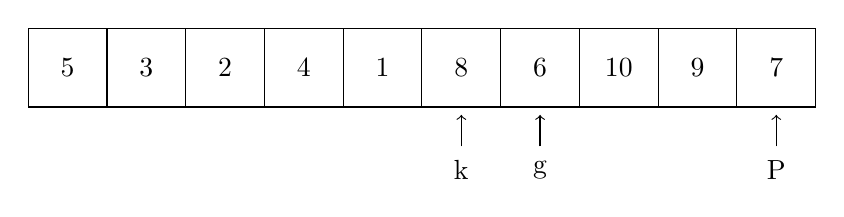
\begin{tikzpicture}
    \foreach \x in {1,...,10}
      \draw (\x,0) +(-.5,-.5) rectangle ++(.5,.5);
      \draw (1,0) node{5};
      \draw (2,0) node{3};
      \draw (3,0) node{2};
      \draw (4,0) node{4};
      \draw (5,0) node{1};
      \draw (6,0) node{8};
      \draw (7,0) node{6};
      \draw (8,0) node{10};
      \draw (9,0) node{9};
      \draw (10,0) node{7};
      \draw [->](10,-1) -- (10,-0.6);
      \draw (10,-1.3) node{P};
      \draw [->](7,-1) -- (7,-0.6);
      \draw (7,-1.3) node{g};
      \draw [->](6,-1) -- (6,-0.6);
      \draw (6,-1.3) node{k};
 \end{tikzpicture}
  \caption{Zweites Paar zum Tauschen}
  \label{quicksortArrayP_k_g_13}
\end{figure}

\begin{figure}
  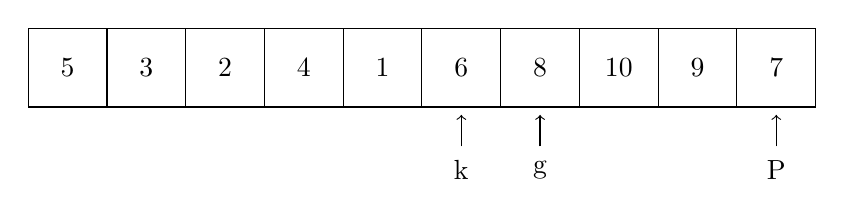
\begin{tikzpicture}
    \foreach \x in {1,...,10}
      \draw (\x,0) +(-.5,-.5) rectangle ++(.5,.5);
      \draw (1,0) node{5};
      \draw (2,0) node{3};
      \draw (3,0) node{2};
      \draw (4,0) node{4};
      \draw (5,0) node{1};
      \draw (6,0) node{6};
      \draw (7,0) node{8};
      \draw (8,0) node{10};
      \draw (9,0) node{9};
      \draw (10,0) node{7};
      \draw [->](10,-1) -- (10,-0.6);
      \draw (10,-1.3) node{P};
      \draw [->](7,-1) -- (7,-0.6);
      \draw (7,-1.3) node{g};
      \draw [->](6,-1) -- (6,-0.6);
      \draw (6,-1.3) node{k};
 \end{tikzpicture}
  \caption{Array, Hilfszeiger haben die Position gewechselt}
  \label{quicksortArrayP_k_g_14}
\end{figure}

Zum Abschluss des Arbeitsschritts wird geprüft, ob die Inhalte an den Positionen P und g getauscht werden müssen. Wenn das Element an der Position g größer ist, als das an P (Bild \ref{quicksortArrayP_k_g_14}), werden die Inhalte ausgetauscht. Damit ist die erste Runde des Algorithmus beendet.

\begin{figure}
  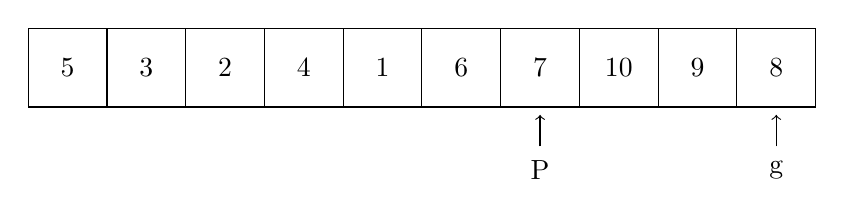
\begin{tikzpicture}
    \foreach \x in {1,...,10}
      \draw (\x,0) +(-.5,-.5) rectangle ++(.5,.5);
      \draw (1,0) node{5};
      \draw (2,0) node{3};
      \draw (3,0) node{2};
      \draw (4,0) node{4};
      \draw (5,0) node{1};
      \draw (6,0) node{6};
      \draw (7,0) node{7};
      \draw (8,0) node{10};
      \draw (9,0) node{9};
      \draw (10,0) node{8};
      \draw [->](10,-1) -- (10,-0.6);
      \draw (10,-1.3) node{g};
      \draw [->](7,-1) -- (7,-0.6);
      \draw (7,-1.3) node{P};
 \end{tikzpicture}
  \caption{Tausch \glq gross\grq \ mit Pivotelement}
  \label{quicksortArrayP_k_g_15}
\end{figure}

\subsubsection{Runde 2}
In der nächsten runde werden die Abschnitte links und rechts von $\text{P}_1$ zu eigenen Teilen, die einzeln betrachtet werden. Im linken Abschnitt wird 6 zum neuen Pivotelement, 8 ist im rechten Abschnitt das neue Pivotelement (Bild \ref{quicksortArrayP_k_g_21}).

\begin{figure}
  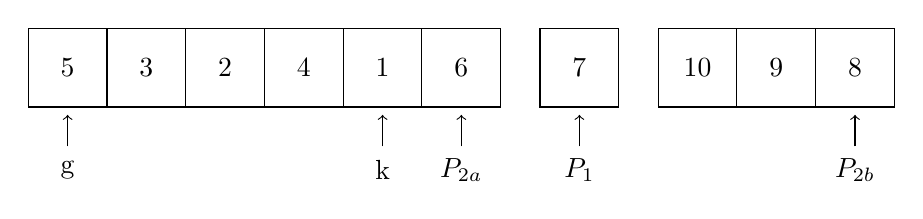
\begin{tikzpicture}
    \foreach \x in {1,...,6}
      \draw (\x,0) +(-.5,-.5) rectangle ++(.5,.5);
    \draw (1,0) node{5};
    \draw (2,0) node{3};
    \draw (3,0) node{2};
    \draw (4,0) node{4};
    \draw (5,0) node{1};
    \draw (6,0) node{6};
    \draw (7, -0.5) rectangle (8, 0.5);
    \draw (7.5,0) node{7};
    \draw (8.5, -0.5) rectangle (9.5, 0.5);
    \draw (9,0) node{10};
    \draw (9.5, -0.5) rectangle (10.5, 0.5);
    \draw (10,0) node{9};
    \draw (10.5, -0.5) rectangle (11.5, 0.5);
    \draw (11,0) node{8};
    \draw [->](6,-1) -- (6,-0.6);
    \draw (6,-1.3) node{$\text{P}_{2a}$};
    \draw [->](11,-1) -- (11,-0.6);
    \draw (11,-1.3) node{$\text{P}_{2b}$};
    \draw [->](5,-1) -- (5,-0.6);
    \draw (5,-1.3) node{k};
    \draw [->](1,-1) -- (1,-0.6);
    \draw (1,-1.3) node{g};
    \draw [->](7.5,-1) -- (7.5,-0.6);
    \draw (7.5,-1.3) node{$\text{P}_1$};
 \end{tikzpicture}
 \caption{Aufteilung, $\text{P}_1$ ist alleine, links und rechts neue Bereiche}
  \label{quicksortArrayP_k_g_21}
\end{figure}

In Runde zwei der Sortierung betrachte ich zuerst den linken Teil und suche hier wieder die Elemente, die kleiner und größer als das Pivotelement sind (Bild \ref{quicksortArrayP_k_g_21}). Da kein Element aus der linken Teilmenge größer als 7 ist, wird hier nicht getauscht.

\begin{figure}
  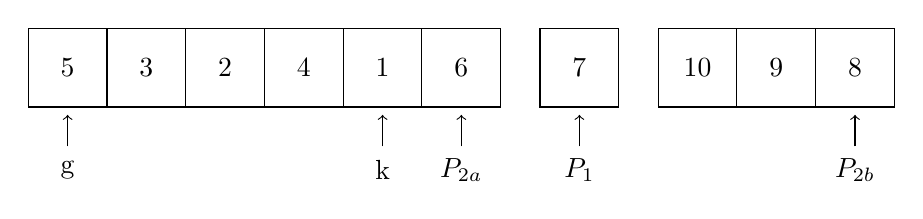
\begin{tikzpicture}
    \foreach \x in {1,...,6}
      \draw (\x,0) +(-.5,-.5) rectangle ++(.5,.5);
    \draw (1,0) node{5};
    \draw (2,0) node{3};
    \draw (3,0) node{2};
    \draw (4,0) node{4};
    \draw (5,0) node{1};
    \draw (6,0) node{6};
    \draw (7, -0.5) rectangle (8, 0.5);
    \draw (7.5,0) node{7};
    \draw (8.5, -0.5) rectangle (9.5, 0.5);
    \draw (9,0) node{10};
    \draw (9.5, -0.5) rectangle (10.5, 0.5);
    \draw (10,0) node{9};
    \draw (10.5, -0.5) rectangle (11.5, 0.5);
    \draw (11,0) node{8};
    \draw [->](6,-1) -- (6,-0.6);
    \draw (6,-1.3) node{$\text{P}_{2a}$};
    \draw [->](11,-1) -- (11,-0.6);
    \draw (11,-1.3) node{$\text{P}_{2b}$};
    \draw [->](5,-1) -- (5,-0.6);
    \draw (5,-1.3) node{k};
    \draw [->](1,-1) -- (1,-0.6);
    \draw (1,-1.3) node{g};
    \draw [->](7.5,-1) -- (7.5,-0.6);
    \draw (7.5,-1.3) node{$\text{P}_1$};
 \end{tikzpicture}
 \caption{Suche links ist abgeschlossen ($5 < 7$)}
  \label{quicksortArrayP_k_g_22}
\end{figure}

Im rechten Teil werden die Elemente 10 und 9 nicht getauscht, da 9 größer als 8 ist. Die zweite Prüfung ($10 > 8$) fällt positiv aus. Daher werden 10 (k) und $P_{2b}$ getauscht.

\begin{figure}
  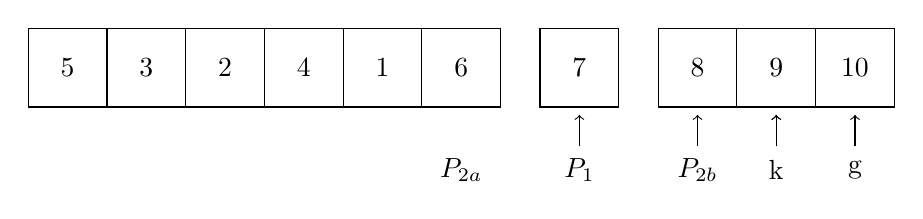
\begin{tikzpicture}
    \foreach \x in {1,...,6}
      \draw (\x,0) +(-.5,-.5) rectangle ++(.5,.5);
    \draw (1,0) node{5};
    \draw (2,0) node{3};
    \draw (3,0) node{2};
    \draw (4,0) node{4};
    \draw (5,0) node{1};
    \draw (6,0) node{6};
    \draw (7, -0.5) rectangle (8, 0.5);
    \draw (7.5,0) node{7};
    \draw (8.5, -0.5) rectangle (9.5, 0.5);
    \draw (9,0) node{8};
    \draw (9.5, -0.5) rectangle (10.5, 0.5);
    \draw (10,0) node{9};
    \draw (10.5, -0.5) rectangle (11.5, 0.5);
    \draw (11,0) node{10};
    \draw [->](10,-1) -- (10,-0.6);
    \draw (6,-1.3) node{$\text{P}_{2a}$};
    \draw [->](9,-1) -- (9,-0.6);
    \draw (9,-1.3) node{$\text{P}_{2b}$};
    \draw [->](10,-1) -- (10,-0.6);
    \draw (10,-1.3) node{k};
    \draw [->](11,-1) -- (11,-0.6);
    \draw (11,-1.3) node{g};
    \draw [->](7.5,-1) -- (7.5,-0.6);
    \draw (7.5,-1.3) node{$\text{P}_1$};
 \end{tikzpicture}
 \caption{Tausch rechts (10 und 8)}
  \label{quicksortArrayP_k_g_23}
\end{figure}

Somit sind 6 und 10 sortiert.

\subsubsection{Rund 3}

\begin{figure}
  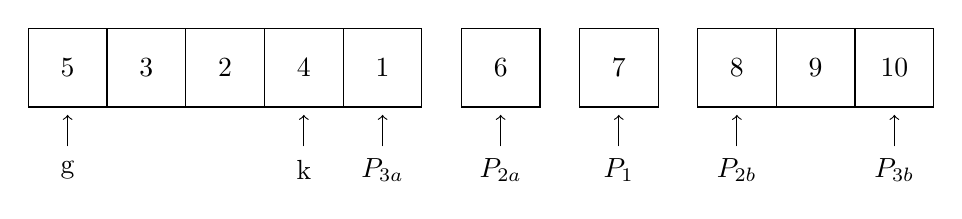
\begin{tikzpicture}
    \foreach \x in {1,...,5}
      \draw (\x,0) +(-.5,-.5) rectangle ++(.5,.5);
    \draw (1,0) node{5};
    \draw (2,0) node{3};
    \draw (3,0) node{2};
    \draw (4,0) node{4};
    \draw (5,0) node{1};
    \draw (6, -0.5) rectangle (7, 0.5);
    \draw (6.5,0) node{6};
    \draw (7.5, -0.5) rectangle (8.5, 0.5);
    \draw (8,0) node{7};
    \draw (9, -0.5) rectangle (10, 0.5);
    \draw (9.5,0) node{8};
    \draw (10, -0.5) rectangle (11, 0.5);
    \draw (10.5,0) node{9};
    \draw (11, -0.5) rectangle (12, 0.5);
    \draw (11.5,0) node{10};
    \draw [->](6.5,-1) -- (6.5,-0.6);
    \draw (6.5,-1.3) node{$\text{P}_{2a}$};
    \draw [->](9.5,-1) -- (9.5,-0.6);
    \draw (9.5,-1.3) node{$\text{P}_{2b}$};
    \draw [->](5,-1) -- (5,-0.6);
    \draw (5,-1.3) node{$\text{P}_{3a}$};
    \draw [->](11.5,-1) -- (11.5,-0.6);
    \draw (11.5,-1.3) node{$\text{P}_{3b}$};
    \draw [->](4,-1) -- (4,-0.6);
    \draw (4,-1.3) node{k};
    \draw [->](1,-1) -- (1,-0.6);
    \draw (1,-1.3) node{g};
    \draw [->](8,-1) -- (8,-0.6);
    \draw (8,-1.3) node{$\text{P}_1$};
 \end{tikzpicture}
 \caption{Runde 3, suche links (g, k, $\text{P}_{3a}$)}
  \label{quicksortArrayP_k_g_31}
\end{figure}

Da keine Zahl kleiner als 1 ist (Bild \ref{quicksortArrayP_k_g_31}), werden hier keine Werte von g und k vertauscht. Lediglich 1 und 5 werden vertauscht. In der rechten Teilmenge ist nur noch 9 als Element vorhanden, hier ist der Vergleich $9 >10$ negativ, daher bleiben die Elemente an der Position stehen. Somit ist auch Runde 3 angeschlossen.

\subsubsection{Runde 4}
\begin{figure}
  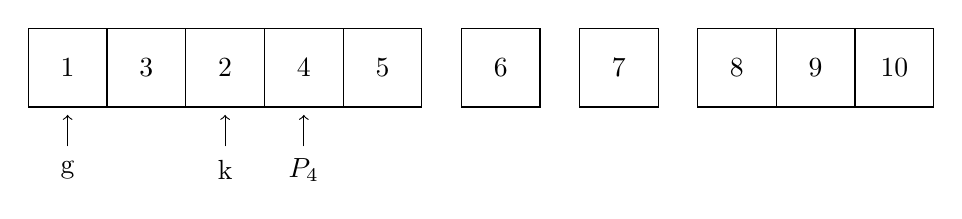
\begin{tikzpicture}
    \foreach \x in {1,...,5}
      \draw (\x,0) +(-.5,-.5) rectangle ++(.5,.5);
    \draw (1,0) node{1};
    \draw (2,0) node{3};
    \draw (3,0) node{2};
    \draw (4,0) node{4};
    \draw (5,0) node{5};
    \draw (6, -0.5) rectangle (7, 0.5);
    \draw (6.5,0) node{6};
    \draw (7.5, -0.5) rectangle (8.5, 0.5);
    \draw (8,0) node{7};
    \draw (9, -0.5) rectangle (10, 0.5);
    \draw (9.5,0) node{8};
    \draw (10, -0.5) rectangle (11, 0.5);
    \draw (10.5,0) node{9};
    \draw (11, -0.5) rectangle (12, 0.5);
    \draw (11.5,0) node{10};
%     \draw [->](6.5,-1) -- (6.5,-0.6);
%     \draw (6.5,-1.3) node{$\text{P}_{2a}$};
%     \draw [->](9.5,-1) -- (9.5,-0.6);
%     \draw (9.5,-1.3) node{$\text{P}_{2b}$};
%     \draw [->](5,-1) -- (5,-0.6);
%     \draw (5,-1.3) node{$\text{P}_{3a}$};
%     \draw [->](11.5,-1) -- (11.5,-0.6);
%     \draw (11.5,-1.3) node{$\text{P}_{3b}$};
    \draw [->](3,-1) -- (3,-0.6);
    \draw (3,-1.3) node{k};
    \draw [->](1,-1) -- (1,-0.6);
    \draw (1,-1.3) node{g};
    \draw [->](4,-1) -- (4,-0.6);
    \draw (4,-1.3) node{$\text{P}_4$};
 \end{tikzpicture}
 \caption{Runde 4, suche links (g, k, $\text{P}_{4}$)}
  \label{quicksortArrayP_k_g_41}
\end{figure}
In Runde 4 wird kein Element vertauscht (Bild \ref{quicksortArrayP_k_g_41}).

\subsubsection{Runde 5}

\begin{figure}
  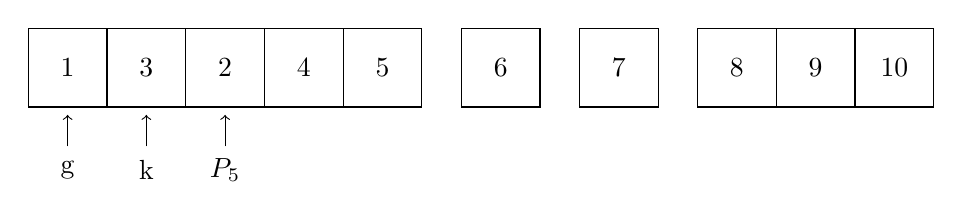
\begin{tikzpicture}
    \foreach \x in {1,...,5}
      \draw (\x,0) +(-.5,-.5) rectangle ++(.5,.5);
    \draw (1,0) node{1};
    \draw (2,0) node{3};
    \draw (3,0) node{2};
    \draw (4,0) node{4};
    \draw (5,0) node{5};
    \draw (6, -0.5) rectangle (7, 0.5);
    \draw (6.5,0) node{6};
    \draw (7.5, -0.5) rectangle (8.5, 0.5);
    \draw (8,0) node{7};
    \draw (9, -0.5) rectangle (10, 0.5);
    \draw (9.5,0) node{8};
    \draw (10, -0.5) rectangle (11, 0.5);
    \draw (10.5,0) node{9};
    \draw (11, -0.5) rectangle (12, 0.5);
    \draw (11.5,0) node{10};
%     \draw [->](6.5,-1) -- (6.5,-0.6);
%     \draw (6.5,-1.3) node{$\text{P}_{2a}$};
%     \draw [->](9.5,-1) -- (9.5,-0.6);
%     \draw (9.5,-1.3) node{$\text{P}_{2b}$};
%     \draw [->](5,-1) -- (5,-0.6);
%     \draw (5,-1.3) node{$\text{P}_{3a}$};
%     \draw [->](11.5,-1) -- (11.5,-0.6);
%     \draw (11.5,-1.3) node{$\text{P}_{3b}$};
    \draw [->](2,-1) -- (2,-0.6);
    \draw (2,-1.3) node{k};
    \draw [->](1,-1) -- (1,-0.6);
    \draw (1,-1.3) node{g};
    \draw [->](3,-1) -- (3,-0.6);
    \draw (3,-1.3) node{$\text{P}_5$};
 \end{tikzpicture}
 \caption{Runde 5, suche links (g, k, $\text{P}_{5}$)}
  \label{quicksortArrayP_k_g_51}
\end{figure}

In Runde 5 (Bild \ref{quicksortArrayP_k_g_51}) werden wieder die Elemente 2 und 3 vertauscht. Bei der Prüfung in Runde 6 (1 und 2) gibt es keine weiteren Vertauschungen, damit ist der Sortieralgorithmus abgeschlossen.

\subsection{Quicksort, zweite Implementierung}
Bei der zweiten Variante wird ebenfalls ein Pivotelement festgelegt und dann alle andere Elemente danach ausgerichtet. Elemente, die kleiner sind kommen auf die linke Seite, Elemente, die größer sind auf die rechte Seite. Anschließend wird der Bereich am Pivotelement getrennt und jeweils der linke und der rechte Bereich als neue Gesamtbereiche betrachtet.
